\documentclass[a4paper, 11pt]{article}
\usepackage[utf8]{inputenc}
\usepackage{amsmath}
\usepackage{array}
\usepackage{listings}
\usepackage{color}
\usepackage{caption}
\usepackage{varioref}
\usepackage[section]{placeins}
\usepackage{comment} % enables the use of multi-line comments (\ifx \fi) 
\usepackage{graphicx}
\usepackage{lipsum} %This package just generates Lorem Ipsum filler text. 
\usepackage{fullpage} % changes the margin
\usepackage{cleveref}
\definecolor{dkgreen}{rgb}{0,0.6,0}
\definecolor{gray}{rgb}{0.5,0.5,0.5}
\definecolor{mauve}{rgb}{0.58,0,0.82}

\DeclareMathOperator*{\argmax}{argmax} % thin space, limits underneath in displays

\newenvironment{conditions}
{\par\vspace{\abovedisplayskip}\noindent\begin{tabular}{>{$}l<{$} @{${}={}$} l}}
	{\end{tabular}\par\vspace{\belowdisplayskip}}

\renewcommand{\lstlistingname}{Algorithm}% Listing -> Algorithm
\renewcommand{\lstlistlistingname}{List of \lstlistingname s}% List of Listings -> List of Algorithms
\crefname{listing}{algorithm}{algorithms}  
\Crefname{listing}{Algorithm}{Algorithms}

\lstset{frame=tb,
	language=Python,
	aboveskip=3mm,
	belowskip=3mm,
	showstringspaces=false,
	columns=flexible,
	basicstyle={\small\ttfamily},
	numbers=left,
	numberstyle=\tiny\color{gray},
	keywordstyle=\color{blue},
	commentstyle=\color{dkgreen},
	stringstyle=\color{mauve},
	breaklines=true,
	breakatwhitespace=true,
	tabsize=3,
	inputencoding=latin1
}

\captionsetup[figure]{skip=0pt}

\begin{document}
	%Header-Make sure you update this information!!!!
	\noindent
	\large\textbf{Homework 1 Report} \hfill \textbf{Piero Macaluso s252894} \\
	\normalsize Machine Learning and Artificial Intelligence 2018/2019 \hfill Due Date: 19/01/2019 \\
	Prof. Barbara Caputo  
	
	\section{Data Preparation}
	\showthe\columnwidth
	
	In this first step, I was asked to prepare the images for the elaboration. The dataset was made by $1087$ samples of $3$x$227$x$227$ size which belong to $4$ visual object categories.
	I extracted all the files in the folder \texttt{PACS\_homework} in the root folder of my workspace then I used $4$ threads (one for every category) each one running \vref{lst:data}.
	I decided to save the images and the labels in two file (\texttt{data.npy} and \texttt{label.npy}) in order to make next loadings faster.
	\lstinputlisting[linerange={62-86},firstnumber=62,label={lst:data},caption={Projection applying PCA}]{../source_code/main.py}
		
	\section{Principal Component Visualization}
	I standardized \texttt{x} using \texttt{StandardScaler} making each feature zero-mean and unit-variance. Then I applied PCA on the normalized X obtaining the projection using all $1087$ PCs as in \vref{lst:pca}.
	I decided to implement a custom function called \texttt{reconstruction()} in order to re-project \texttt{x\_t} using first $60$, $6$, $2$ and last $6$ principal component (PC) and visualize the reconstructed images with \texttt{show\_reconstruction()} function as you can see in \vref{lst:reconstruction}.
	
	\lstinputlisting[float,linerange={249-256},firstnumber=249,label={lst:pca},caption={Applying PCA of sklearn}]{../source_code/main.py}
	
	\lstinputlisting[float,linerange={142-180},firstnumber=142,label={lst:reconstruction},caption={Re-projection on a specific range of components}]{../source_code/main.py}
	
	\subsection{Comments about re-projections}
	I tried to re-project a series of images from different categories and I obtained the results in \vref{fig:dog1,fig:guitar1,fig:house1,fig:person1}.
	
	As we can see, we are able to distinguish some coarse details of the original images in the re-projections with 60PC because these have a cumulative variance of approximately $77\%$ but $6$PC and $2$PC plots has lower variances because of the reduced number of PC used to re-project.
	
	The "Last $6$PC" one has very low variance (approximately $0\%$), instead. I did expect this last result because of PCA transformation: PCs are sort in descending order of variance, so last PCs can not be able to describe correctly the whole dataset.
	
	I noticed that all "Last $6$PC" plots describe the shape of a person: this is probably because we have different amount of images for each category and people ones are the majority. Indeed, the dataset is composed by $189$ dogs ($\approx17\%$), $186$ guitars ($\approx17\%$), $280$ houses ($\approx26\%$) and $432$ people ($\approx40\%$).
	
	Furthermore, the great part of people images are from the same point of view (frontal) in contrast to the other ones where we have different points of view, numbers and rotation: maybe this could be another underlying cause.
		
	\begin{figure}[ht!]
		\centering
		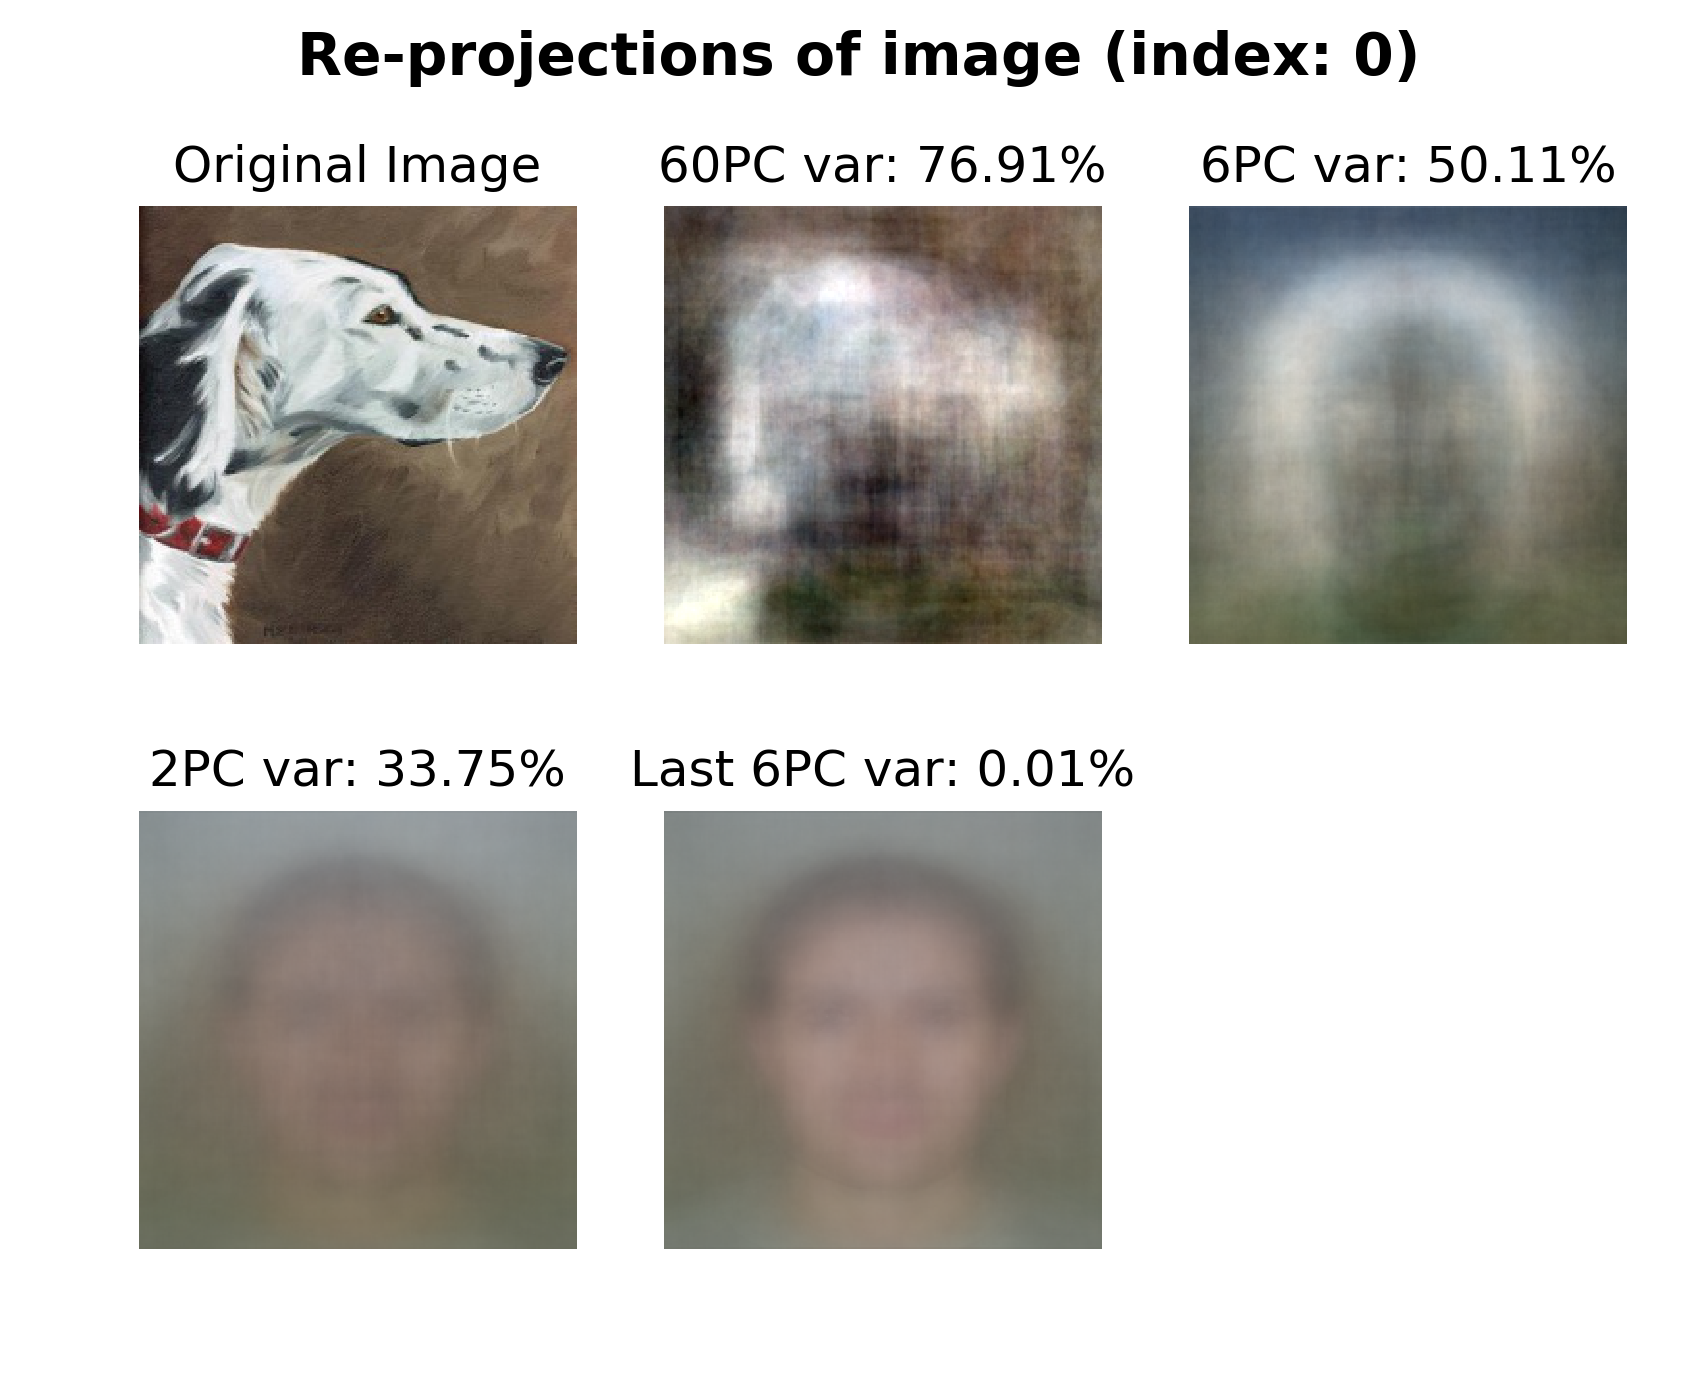
\includegraphics[height=0.5\paperwidth]{img/fig01a.png}
		\caption{Re-projections of a dog image}
		\label{fig:dog1}
	\end{figure}
	\begin{figure}[ht!]
		\centering
		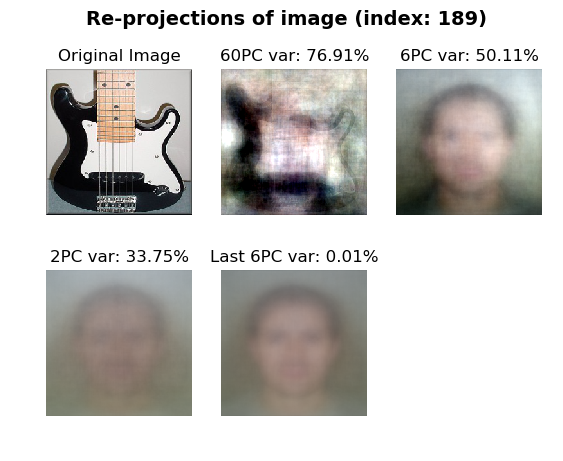
\includegraphics[height=0.5\paperwidth]{img/fig01b.png}
		\caption{Re-projections of a person image}
		\label{fig:guitar1}
	\end{figure}
	\begin{figure}[ht!]
		\centering
		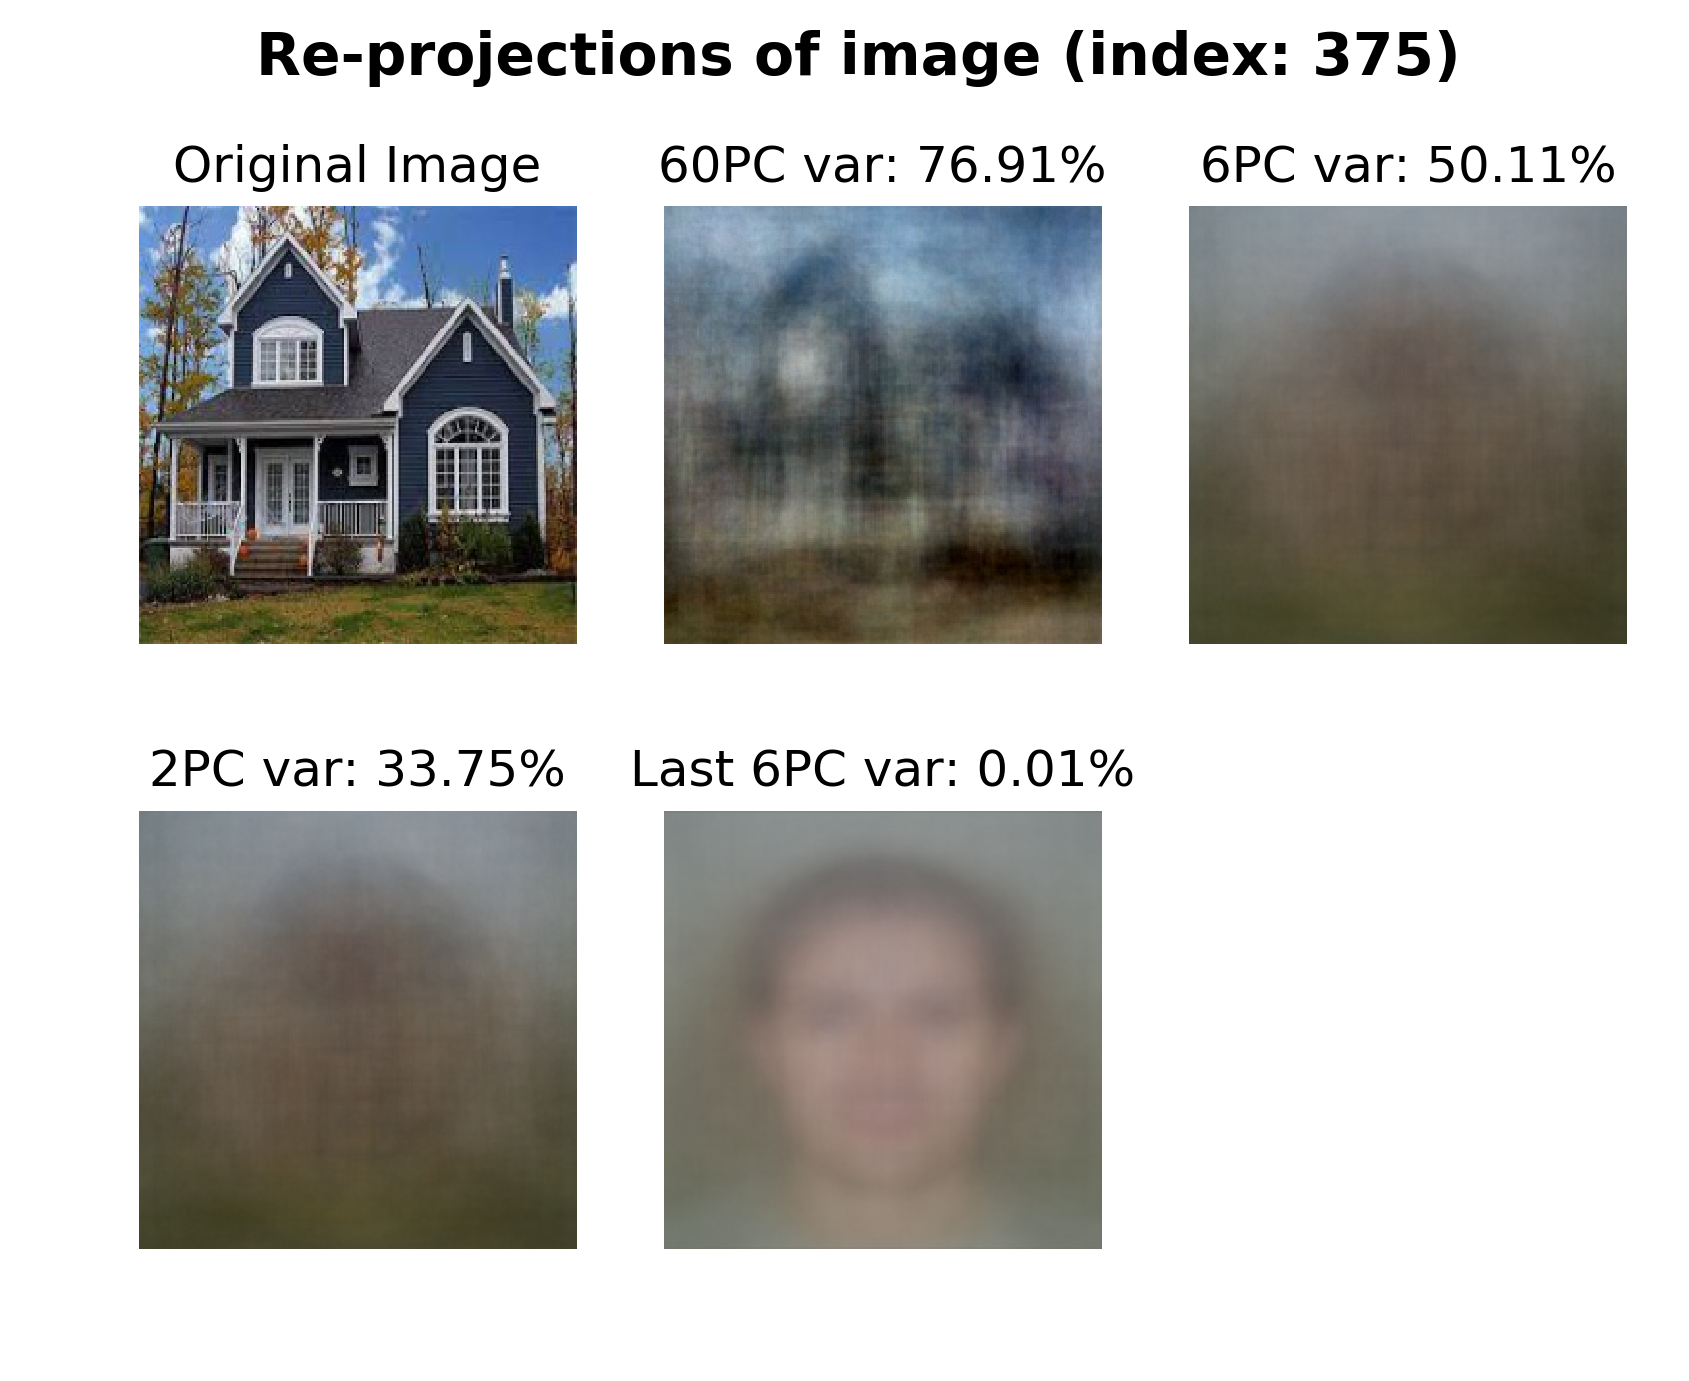
\includegraphics[height=0.5\paperwidth]{img/fig01c.png}
		\caption{Re-projections of a person image}
		\label{fig:house1}
	\end{figure}
	\begin{figure}[ht!]
		\centering
		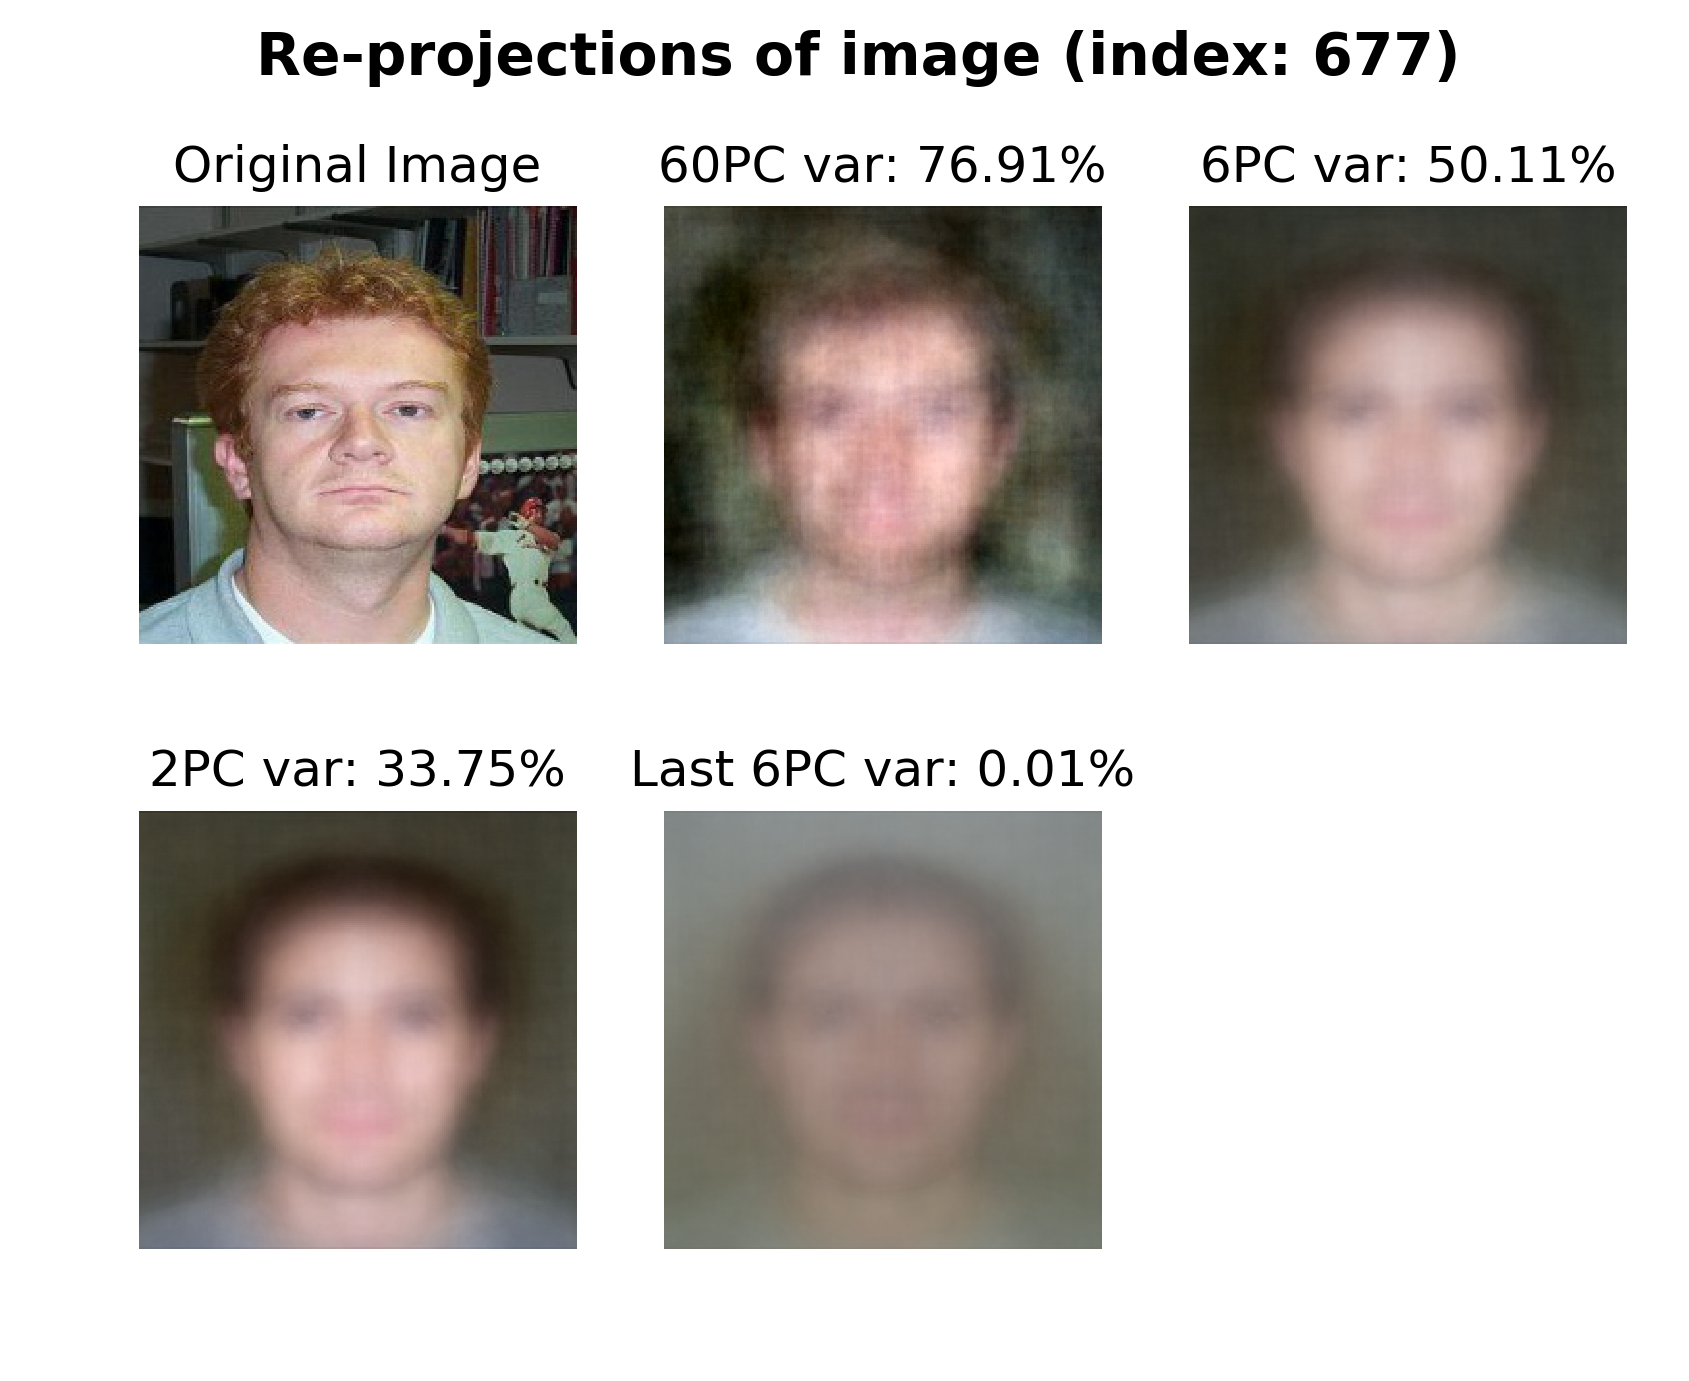
\includegraphics[height=0.5\paperwidth]{img/fig01d.png}
		\caption{Re-projections of a person image}
		\label{fig:person1}
	\end{figure}
	
	\FloatBarrier
	
	\subsection{Comments about scatter and variance plots}
	I produced scatter plot using different combination of PCs as we can see in \vref{fig:scatter1,fig:scatter2,fig:scatter3,fig:scatter4}.
	
	In \vref{fig:scatter1} there is a projection on $1$st and $2$nd PC: it is easy to find an area for \textit{person} and \textit{house} classes, while \textit{guitar} and \textit{dog} ones have a wider distribution on the plot.
	
	In \vref{fig:scatter2,fig:scatter3} there are a $3$rd and $4$th PC projection and a $10$th and $11$th PC one: in this case it seems more difficult to find crowded areas and almost isolated of a single category.
	
	I noticed that the range of coordinates in the graphs was about inversely proportional to the position of PC used, or, better, that the points in the scatter plot were getting closer and closer to the mean (which is $0$ because of normalization) resulting in \textbf{decreased variance}. This can be explained from theoretical perspective because, in the definition of PCA transformation, the first principal component has the \textbf{largest possible variance}, and each succeeding component in turn has the highest variance possible under the constraint that it is \textbf{orthogonal} to the preceding components.
	
	Plotting the cumulative sum of variance ratio (provided in the PCA of \texttt{sklearn}) may be useful in order to decide how many components are necessary to preserve data without much distortion. In general, there is not a right and unique way to select the \textit{correct} number of Principal Components, but in this context we can analyze the graph \vref{fig:variance} and select a number of PC characterized by a cumulative sum of variance ratio higher than a specific threshold (e.g., $95\%$).
	
	\begin{figure}[ht!]
		\centering
		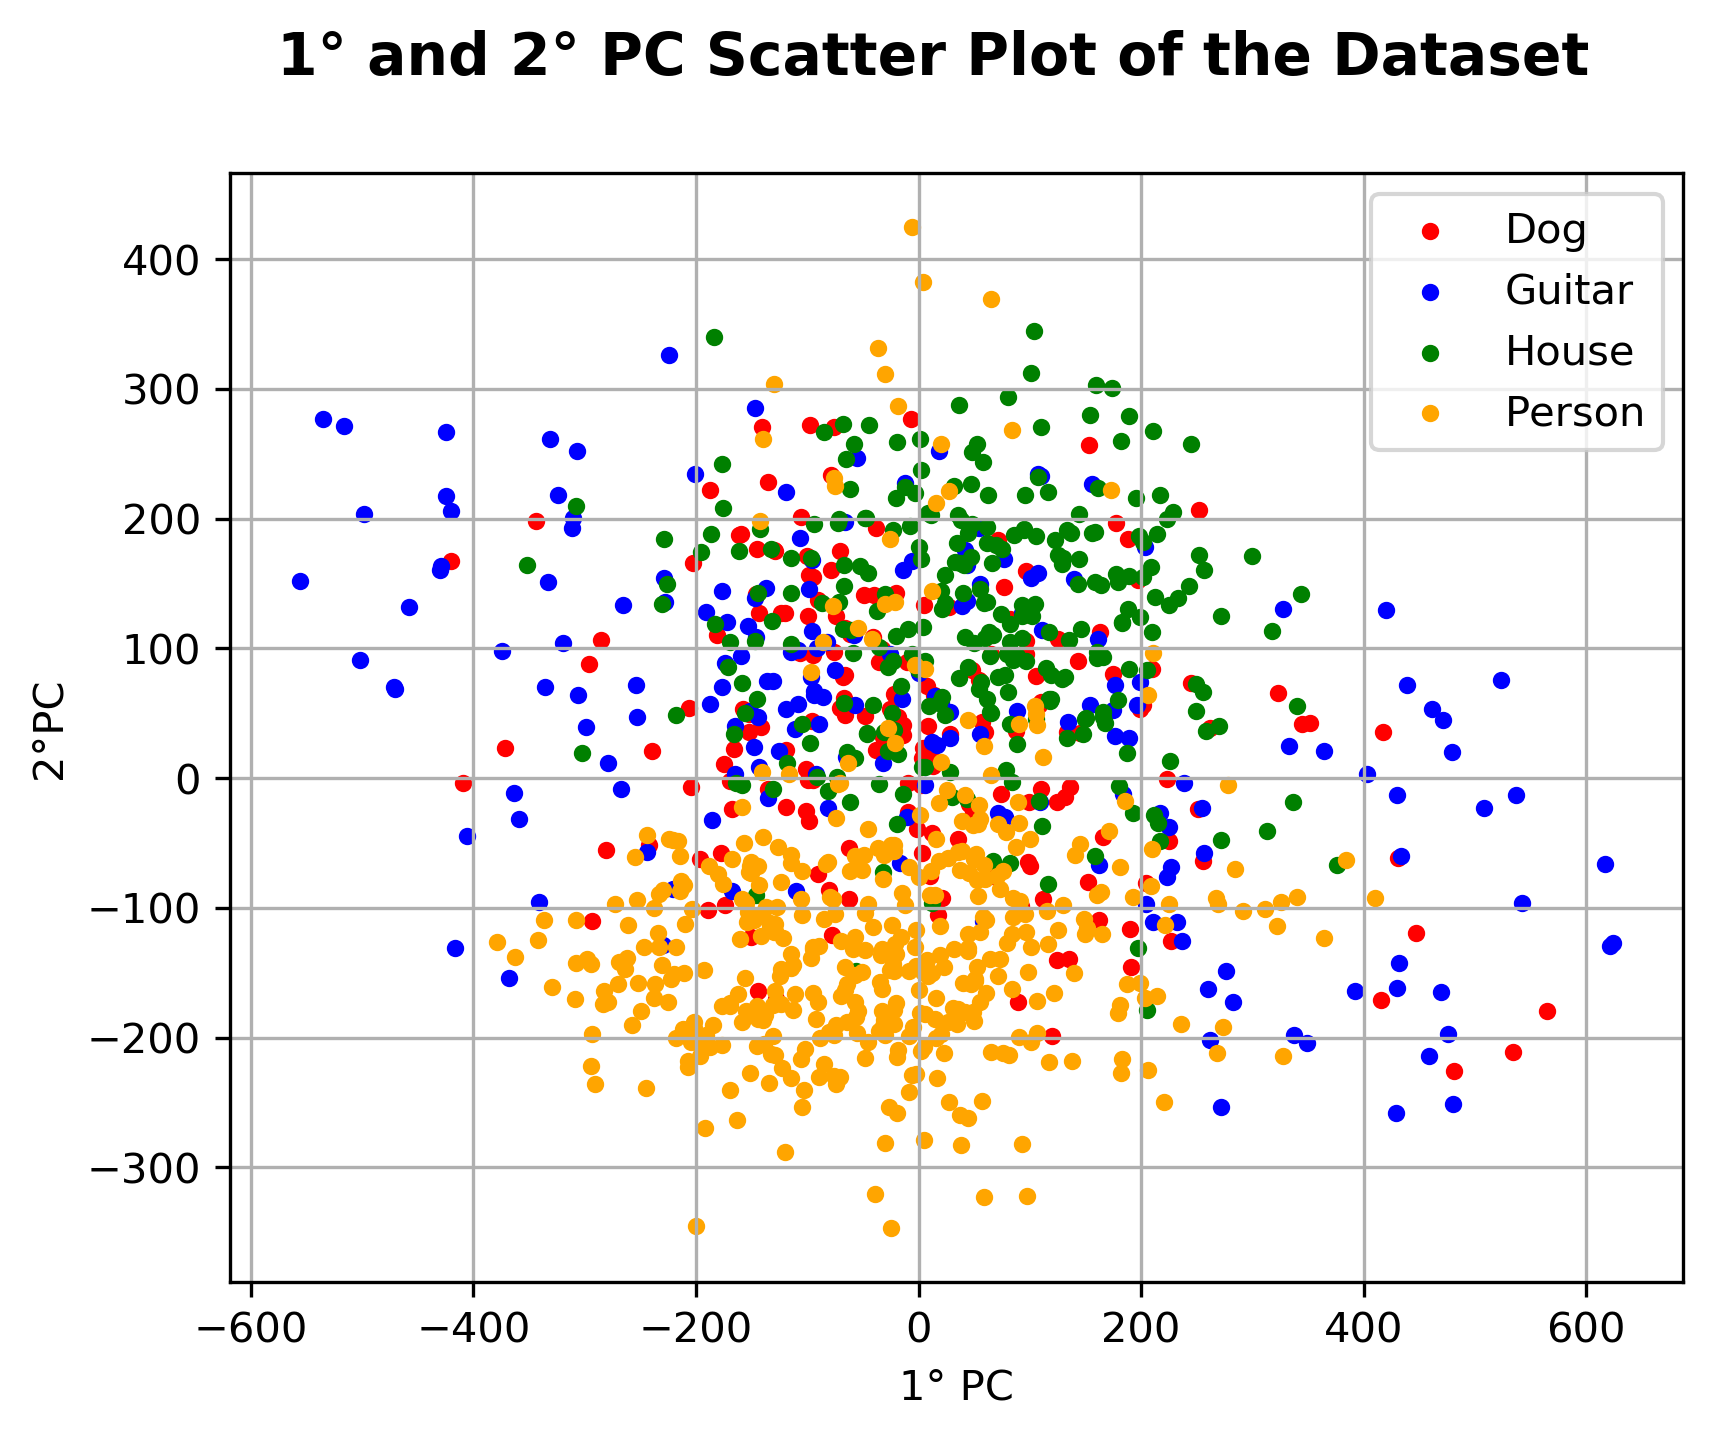
\includegraphics[height=0.5\paperwidth]{img/fig02a.png}
		\caption{Projection on $1$st and $2$nd PC}
		\label{fig:scatter1}
	\end{figure}
	\begin{figure}[ht!]
		\centering
		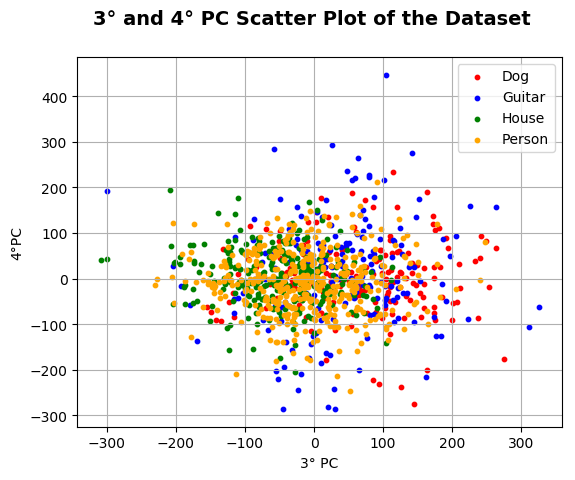
\includegraphics[height=0.5\paperwidth]{img/fig02b.png}
		\caption{Projection on $3$rd and $4$th PC}
		\label{fig:scatter2}
	\end{figure}
	\begin{figure}[ht!]
		\centering
		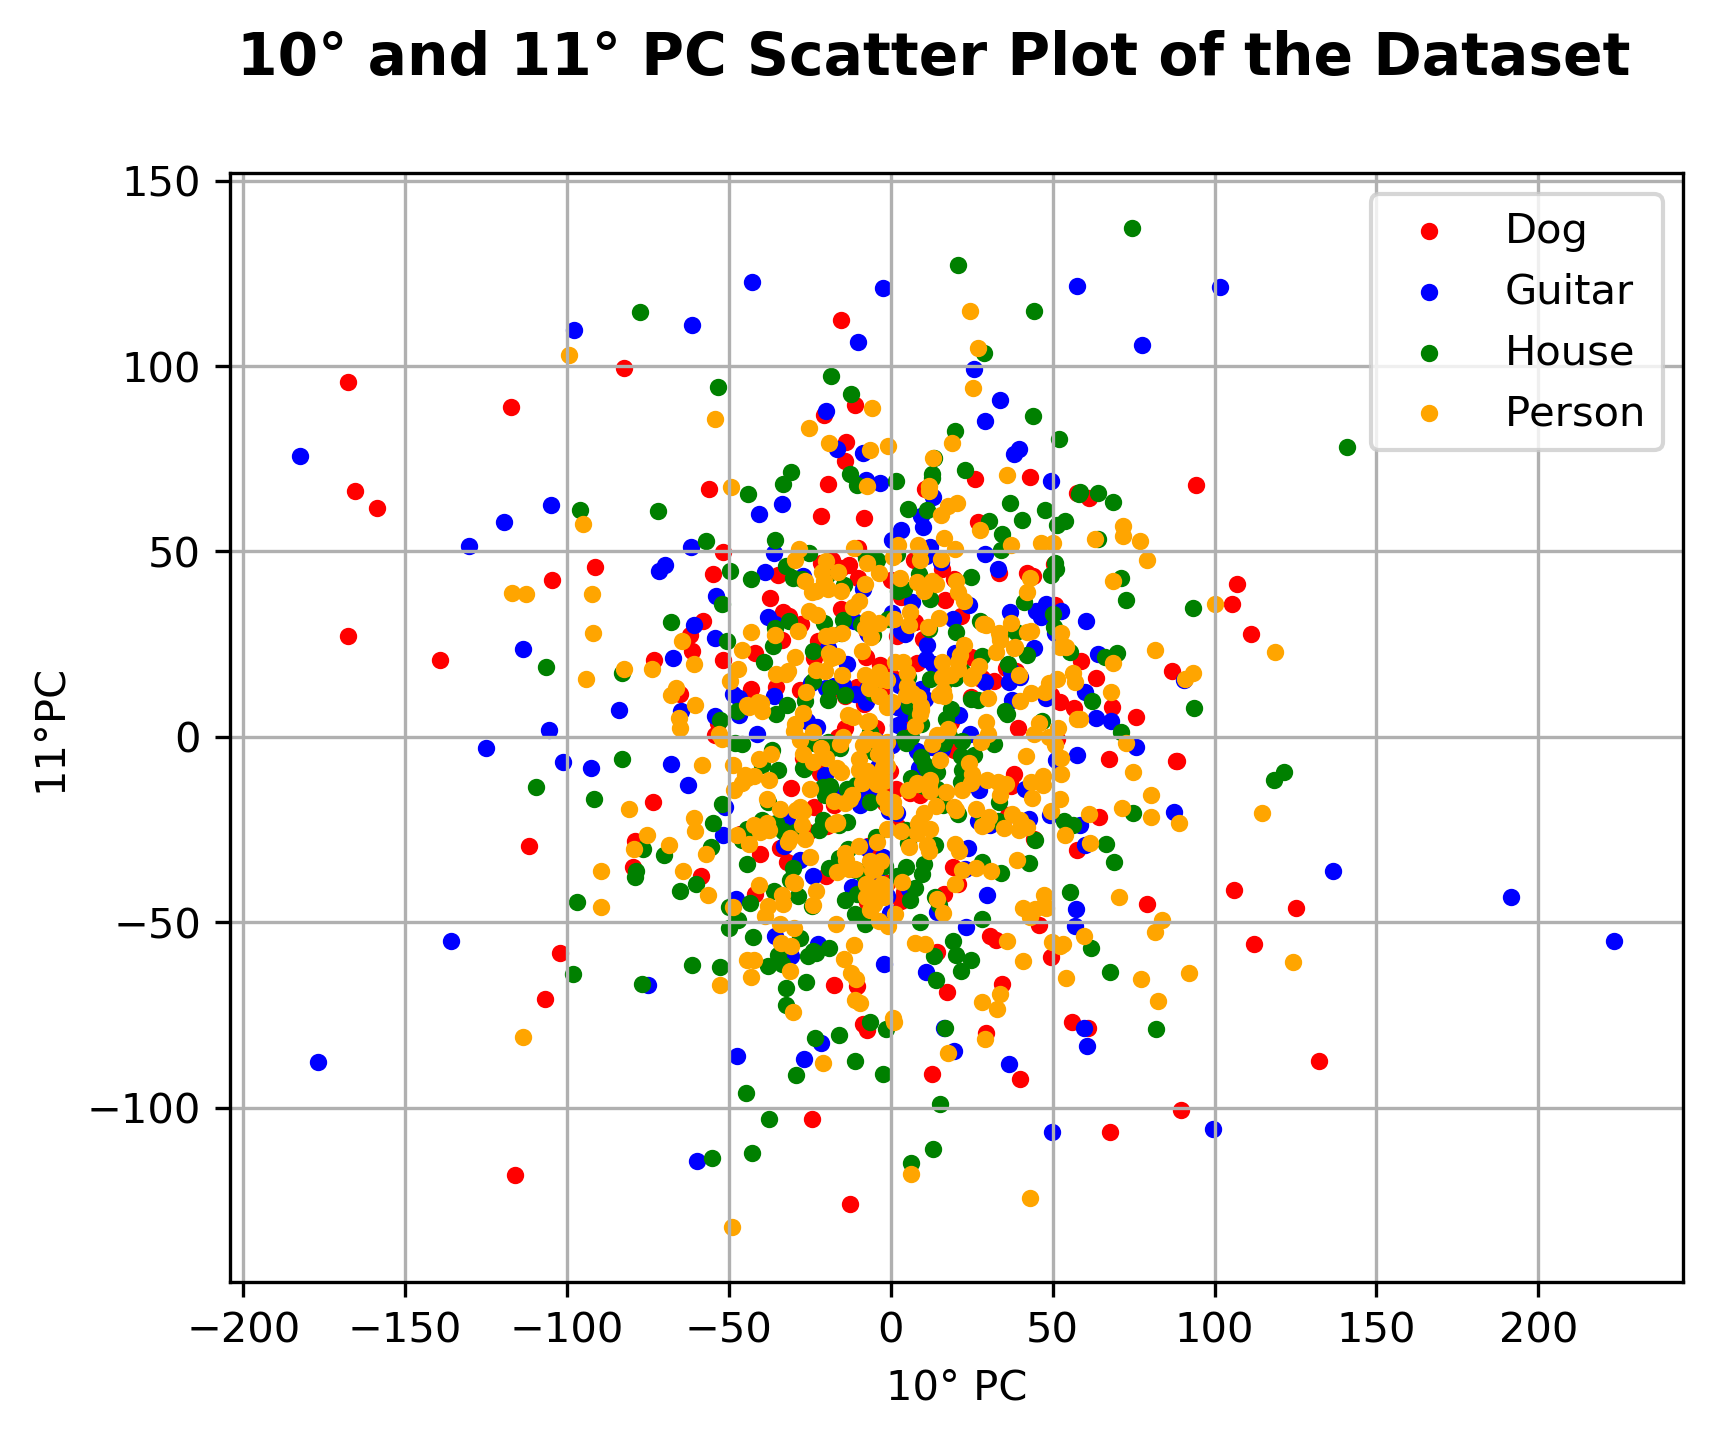
\includegraphics[height=0.5\paperwidth]{img/fig02c.png}
		\caption{Projection on $10$th and $11$th PC}
		\label{fig:scatter3}
	\end{figure}
	\begin{figure}[ht!]
		\centering
		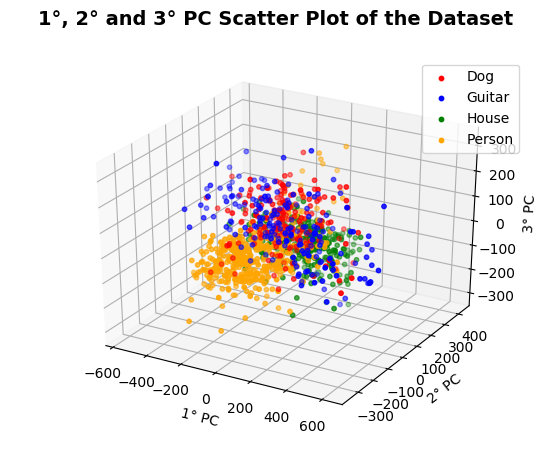
\includegraphics[height=0.5\paperwidth]{img/fig02d.png}
		\caption{Projection on $1$st, $2$nd and $3$rd PC}
		\label{fig:scatter4}
	\end{figure}
	\begin{figure}[ht!]
		\centering
		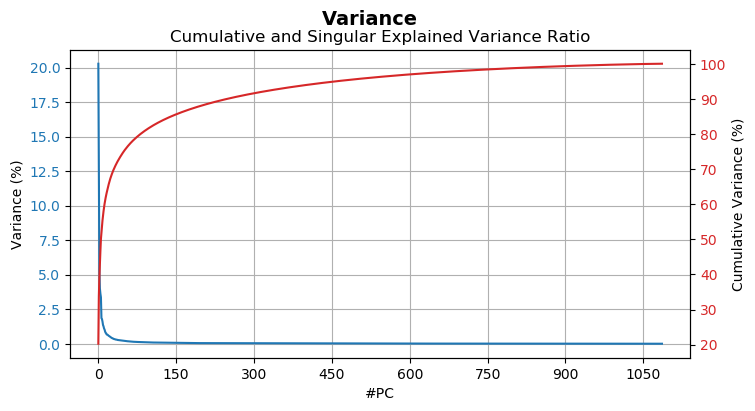
\includegraphics[height=0.4\paperwidth]{img/fig03.png}
		\caption{Variance and Cumulative Variance}
		\label{fig:variance}
	\end{figure}
	
	
	\section{Classification}
		
	The formulation of Na\"ive Bayes is described in \cref{eq:1}.
	\begin{equation} \label{eq:1}
		\hat{y}=\argmax_{i \in \{1,\dots,k\}} p ( y_i \mid x_1, \dots, x_d) = \argmax_{i \in \{1,\dots,k\}}\overbrace{p(y_i)}^{Prior} \prod_{j=1}^{d}\overbrace{p(x_j\mid y_i)}^{Likelihood}
	\end{equation}
	where
	\begin{conditions}
		\hat{y_i}	&	predicted label \\
		y_i			&	$i$-th label with $i \in \{1,\dots,k\}$\\
		x_j			&  	$j$-th example with $j \in \{1,\dots,d\}$   \\   
		p(x\mid y) 	&	Gaussian
	\end{conditions}
	
	Firstly, I splitted randomly \texttt{x\_n} (\texttt{x} standardized) and the labels in \textbf{training} ($75$\%) and \textbf{test set} ($25$\%), then I applied \texttt{GaussianNB} of \texttt{sklearn} obtaining an accuracy of $\boldsymbol{75\%}$.
	
	After that, I splitted in the same way \texttt{x\_t} (the projection of \texttt{x\_n} obtained from PCA transformation) and I used these sets to train and test the classifier first using the data projected on $1$st and $2$nd PC and finally the one projected on $3$rd and $4$th PC. In the first case the accuracy was $\boldsymbol{59.19\%}$, while in the second one was $\boldsymbol{48.53\%}$.
	
	I plotted \textbf{decision boundaries} of the classifier and the projection of the whole dataset for both cases as we can see in \vref{fig:class1,fig:class2}.
	
	
	Comparing accuracy results, we can conclude that classifications done after the application of PCA are worse than the one on the original normalized dataset. Furthermore, the accuracy of classifier on $1$st and $2$nd PC is higher than the one of classifier on $3$rd and $4$th PC, probably because of the different variance that a specific component can describe.
	This may be due to the fact that reducing dimensionality may discard important information useful to discriminate a class from the others in a classifier.
	
	\lstinputlisting[float,linerange={183-224},firstnumber=183,label={lst:classification},caption={Classification and Plot of Decision boundaries}]{../source_code/main.py}

	\begin{figure}[ht!]
		\centering
		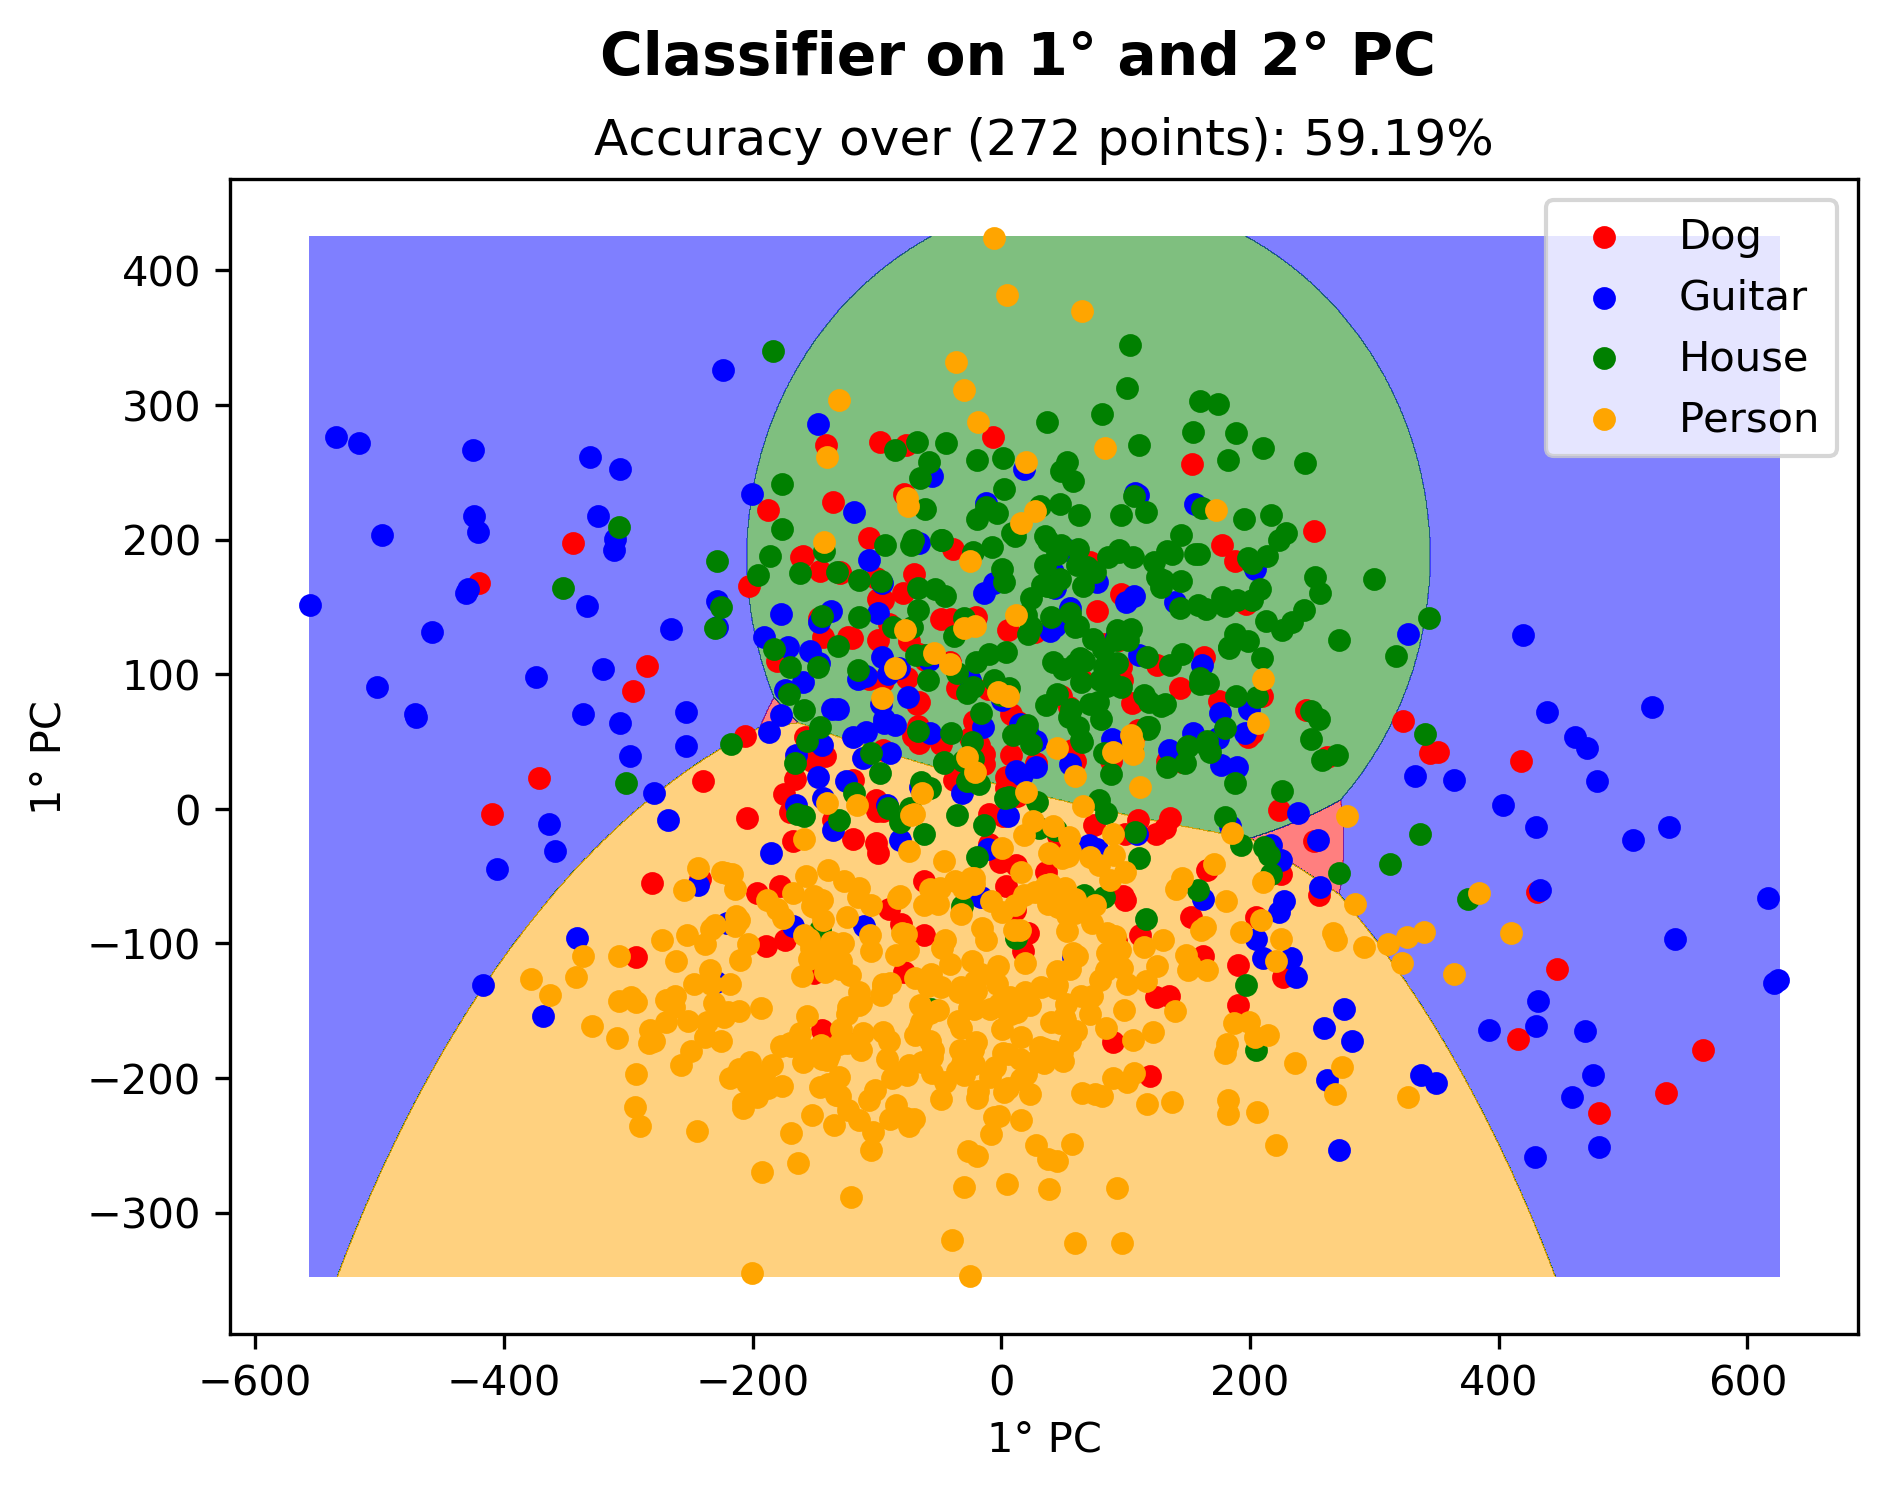
\includegraphics[height=0.52\paperwidth]{img/fig04.png}
		\caption{Decision boundaries of first classifier on $1$st and $2$nd PC}
		\label{fig:class1}
	\end{figure}
	\begin{figure}[ht!]
		\centering
		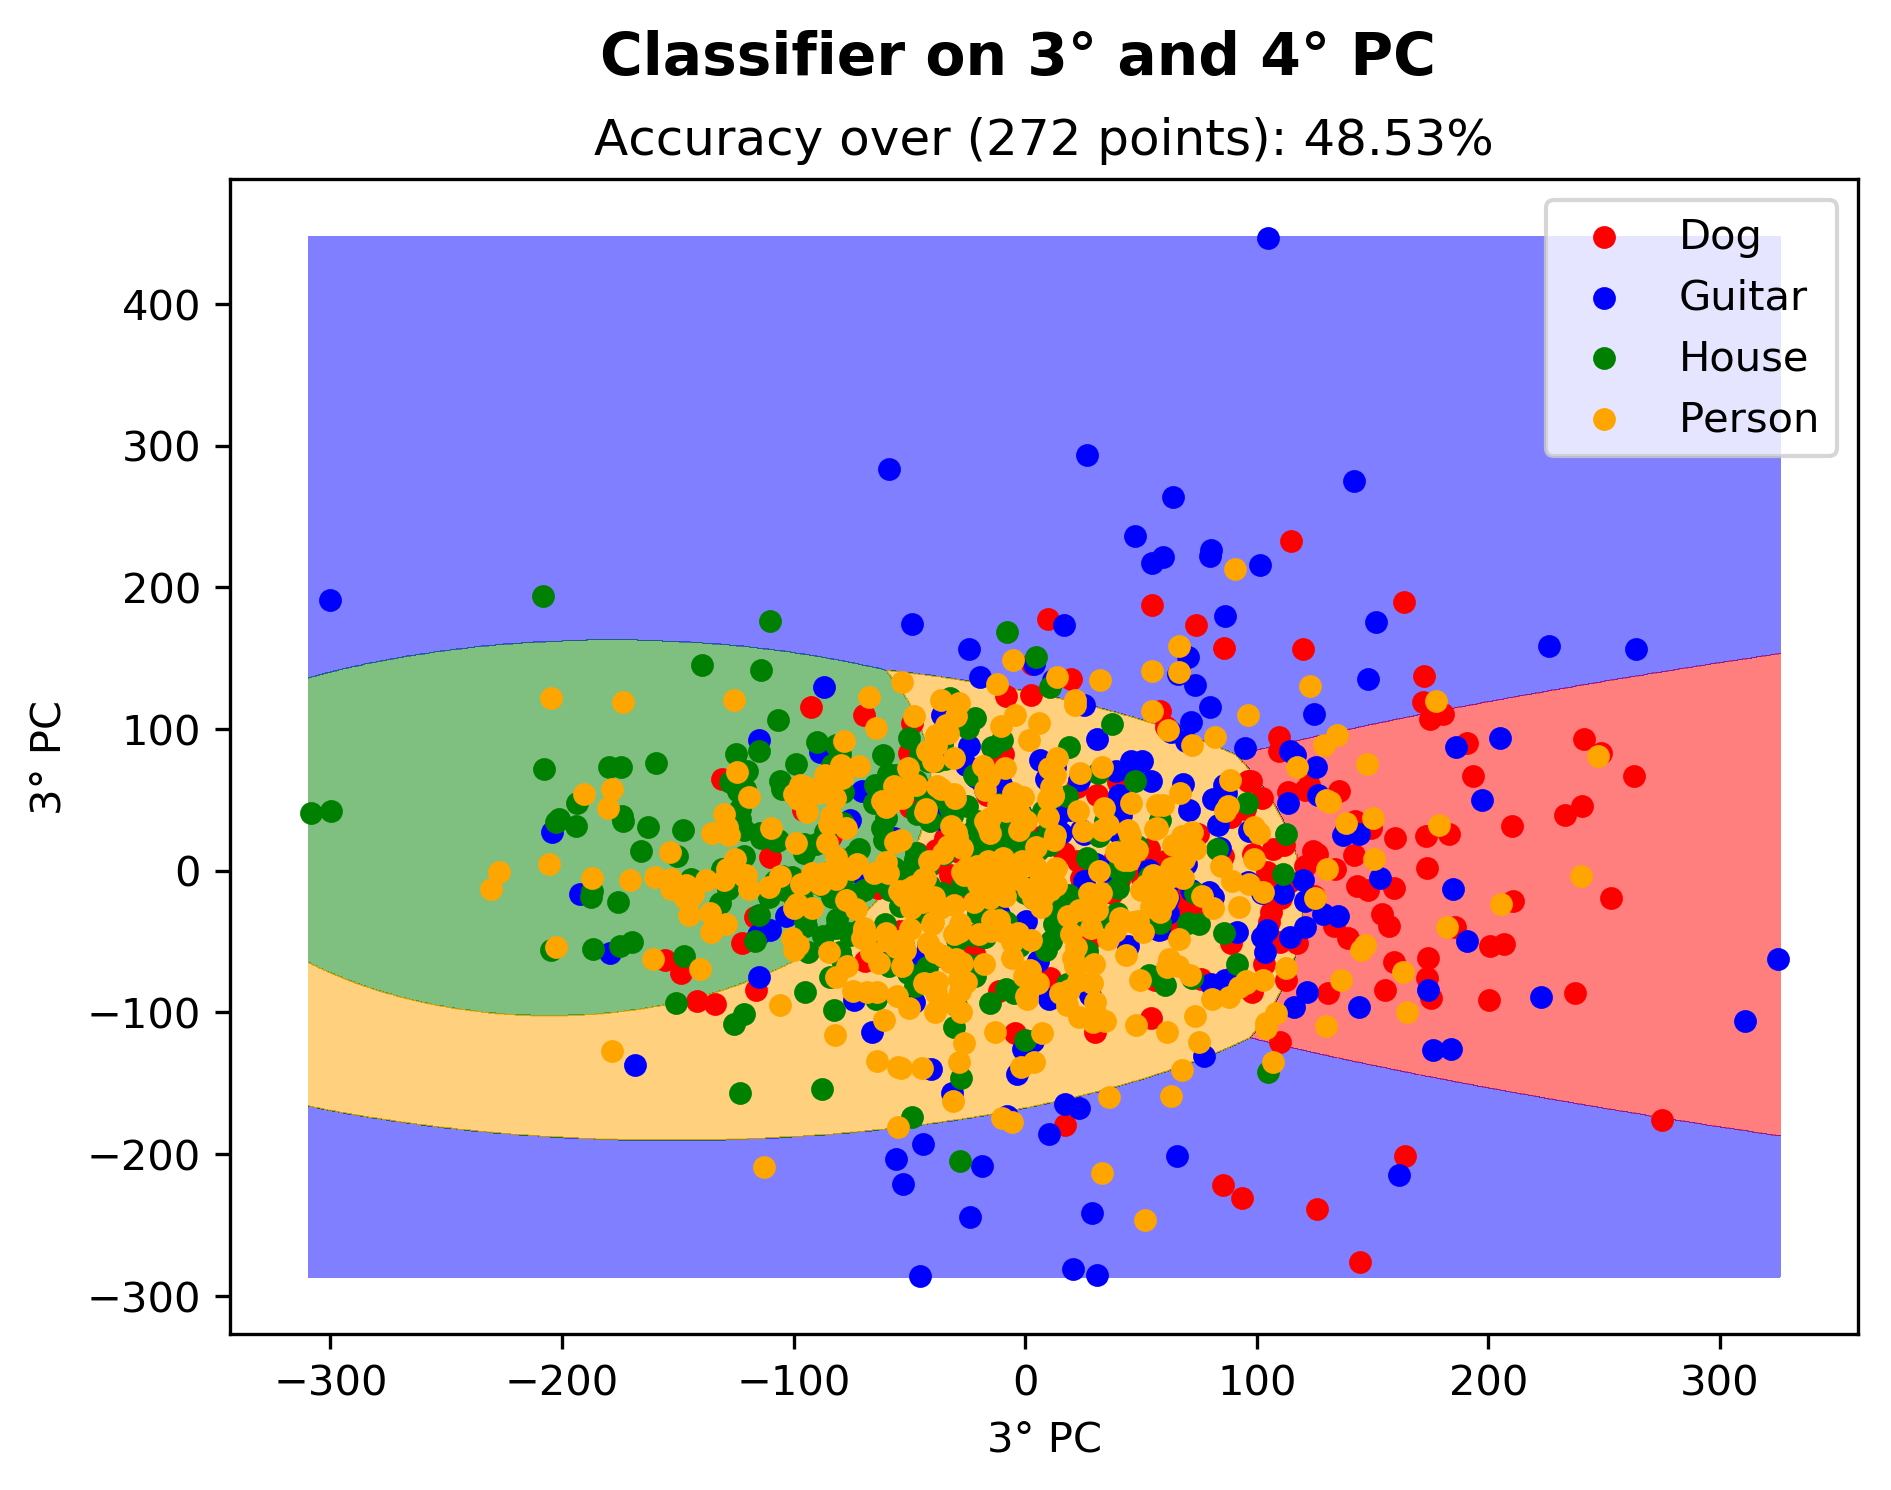
\includegraphics[height=0.52\paperwidth]{img/fig05.png}
		\caption{Decision boundaries of classifier on $3$rd and $4$th PC}
		\label{fig:class2}
	\end{figure}
	
	
	\section{Code Execution}
	\subsection{Requirements}
	\begin{itemize}
		\item Python 3
		\item All dependencies in \texttt{requirements.txt}.
		
		\texttt{\$ pip install -r requirements.txt} to install them
	\end{itemize}
	\subsection{Usage}
	\begin{itemize}
		\item \texttt{\$ python main.py -n <PACS\_homework folder>}
		
		Loads Image from the specified \texttt{<PACS\_homework folder>} and execute the code
		
		\item \texttt{\$ python main.py -s <PACS\_homework folder>}
		
		Loads Image from the specified \texttt{<PACS\_homework folder>} and save files in \texttt{data.npy} and \texttt{label.npy} for faster next execution before executing the code
		
		\item \texttt{\$ python main.py -l <data.npy file> <label.npy file> }
		
		Loads Image from \texttt{data.npy} and \texttt{label.npy} files and execute the code
	
	\end{itemize}
	\subsection{Reproducibility}
	In order to reproduce the same data for this experiment you have to change the global variable \texttt{r\_state} (line) from \texttt{None} to $252894$ which is my badge number.

	\section*{Attachments}
	%Make sure to change these
	\begin{itemize}
		\item Source Code:
		\begin{itemize}
			\item \texttt{main.py}
			\item \texttt{requirements.txt}
		\end{itemize}
	\end{itemize}
	%\fi %comment me out
	
	
	
%	\begin{thebibliography}{9}
%		\bibitem{Robotics} Fred G. Martin \emph{Robotics Explorations: A Hands-On Introduction to Engineering}. New Jersey: Prentice Hall.
%		\bibitem{Flueck}  Flueck, Alexander J. 2005. \emph{ECE 100}[online]. Chicago: Illinois Institute of Technology, Electrical and Computer Engineering Department, 2005 [cited 30
%		August 2005]. Available from World Wide Web: (http://www.ece.iit.edu/~flueck/ece100).
%	\end{thebibliography}
	
\end{document}
